\documentclass[11pt, a4paper]{report}

% Page styling
\usepackage{amssymb,graphicx,color}
\usepackage{amsfonts}
\usepackage{extsizes}
\usepackage{latexsym}
\usepackage[a4paper,margin=3cm]{geometry}
\usepackage{changepage}
\usepackage{mathptmx}

% Spacing
\usepackage{setspace}
\setstretch{1.05}

% Tables
\usepackage{multirow, multicol}
\usepackage{booktabs}
\setlength{\columnsep}{1cm}

% Custom theorems
\usepackage[font=small, labelfont=bf]{caption}
\usepackage[protrusion=true, expansion=true]{microtype}
\usepackage{sectsty}
\usepackage{url, lipsum}
\usepackage{amsthm}

\usepackage{hyperref}

\theoremstyle{definition}
\newtheorem{theorem}{THEOREM}
\newtheorem{lemma}[theorem]{LEMMA}
\newtheorem{corollary}[theorem]{COROLLARY}
\newtheorem{proposition}[theorem]{PROPOSITION}
\newtheorem{remark}[theorem]{REMARK}
\newtheorem{definition}[theorem]{DEFINITION}
\newtheorem{fact}[theorem]{FACT}
\newtheorem{example}[theorem]{EXAMPLE}
\newtheorem{property}[theorem]{PROPERTY}

% Positioning figures
\usepackage{float}
\usepackage[demo]{graphicx}
\usepackage{subfig}

% Equations
\usepackage{amsmath}

% Code
\usepackage{fancyvrb}
\usepackage{listings}
\lstset{basicstyle=\ttfamily, keywordstyle=\bfseries}

% Citations
\usepackage{biblatex}
\addbibresource{citations.bib}

% Spacing
\newcommand{\HRule}[1]{\rule{\linewidth}{#1}}
\setcounter{tocdepth}{5}
\setcounter{secnumdepth}{5}
\usepackage{titlesec}
\titleformat{\chapter}[display]
{\normalfont\huge\bfseries}{\chaptertitlename\ \thechapter}{20pt}{\Huge}
\titlespacing*{\chapter}{0pt}{0pt}{20pt}


%----------------------------------------------------------------------------------
% Title Page
%----------------------------------------------------------------------------------
\title{{\vspace{-2in}
\includegraphics[scale=0.4]{docs/Project Report/Media/ucl_logo.png}}\\
\vspace{2cm}
\begin{adjustwidth}{1cm}{1cm}
    \centering
    \Huge Robust Robotic Grasping Utilising Touch Sensing
\end{adjustwidth}}
\\
\date{Submission date: \today}
\author{Koo Ho Tin Justin\thanks{
{\bf Disclaimer:}
This report is submitted as part requirement for the BSc degree in Computer Science at UCL. It is
substantially the result of my own work except where explicitly indicated in the text.
\emph{Either:} The report may be freely copied and distributed provided the source is explicitly acknowledged
\newline  %% \\ messes it up
\emph{Or:}\newline
The report will be distributed to the internal and external examiners, but thereafter may not be copied or distributed except with permission from the author.}
\\ \\
BSc Computer Science\\ \\
Supervisors: Prof. Marc Deisenroth, Dr. Yasemin Bekiroglu}


\begin{document}
\onehalfspacing
\maketitle
\pagenumbering{roman}
\setcounter{page}{i}
%----------------------------------------------------------------------------------
% Abstract
%----------------------------------------------------------------------------------
\begin{abstract}
Robotic grasp synthesis has been studied extensively as robotic grasping skills have a significant impact on the success of subsequent manipulation tasks. Various approaches have been proposed for robotic grasp planning, with different assumptions regarding the available information about the type of objects in question (known, unknown, familiar). These approaches range from heuristic rules, designing simplifying hand models, to completely end-to-end systems inferring grasp parameters from raw data.\\

However, the majority of these approaches do not address robustness in grasping, which refers to the ability of a robot to perform a grasping task consistently and accurately even in the case of unexpected disturbances or large degree of errors in perception. There are several fundamental problems that need to be addressed for achieving better robustness in grasping tasks. These include mainly dealing with uncertainties in sensing, actuation and the perceptual data.\\

In this project, we study how to build a robust learning framework that can be employed to construct robust grasp configurations using multi-modal data, e.g. tactile, and visual. The project addresses the following main issues with the robotic grasping systems: a) balancing the trade-off between data representation and data dimensionality; b) analyzing the modelling effects of different modalities, e.g. tactile and visual, and features to capture the underlying characteristics of the overall grasping process; c) a correction policy that relies on assessing grasp success before further manipulation using perceptual data, to choose the right grasping configuration.
\end{abstract}


%----------------------------------------------------------------------------------
% Acknowledgements
%----------------------------------------------------------------------------------
\renewcommand\abstractname{Acknowledgments}
\begin{abstract}
    
\end{abstract}


%----------------------------------------------------------------------------------
% Contents
%----------------------------------------------------------------------------------
\tableofcontents


%----------------------------------------------------------------------------------
% Chapter 1: Introduction
%----------------------------------------------------------------------------------
\chapter{Introduction}
\label{chap:1}
\pagenumbering{arabic}
\setcounter{page}{1}


\section{Outline of Problem}
\label{sec:1.1}
Humans are able to grasp objects seemingly intuitively. We can efficiently identify and reach for objects, adjust our finger placements and optimally balance contact forces through the coordination of our wrists, arms, and shoulders when we approach and lift objects. Our sense of touch plays a major role, providing us with information about the object's size, shape, texture, weight, and other physical properties. This information is processed by our brains, giving us instructions on how to adjust our grasp pose and apply the appropriate amount of force needed to pick up the object. Without the sense of touch, grasping objects would be much more difficult and less efficient. Therefore, incorporating touch sensing into robotic grasping can help robots better identify and adjust to objects, making them more effective in interacting with the physical world.\\

Recent advancements in machine learning, computer vision, and robotics have led to remarkable progress in the field of robotic grasping. This technology holds great promise for a range of applications, including manufacturing, warehouse automation, and household robotics. However, little work has been done on increasing robustness in grasping systems that utilise multi-modal (tactile and visual) data.\\

Robustness in a robotic grasping system refers to its versatility of accurately recognising and grasping objects with varying geometric features (width, depth, curvature, etc) and its ability to successfully grasp the objects. Robustness is increasingly becoming a vital factor in the study of grasp stability and quality, however, incorporating robustness makes it practically difficult to design a single gripper that can effectively grasp all objects. As a result, researchers and engineers have developed dedicated grippers tailored to specific grasping tasks or types of objects.\\

However, developing a robust and efficient grasping system present several challenges. One major hurdle is the incorporation of touch sensing into robotic grasping, which is hindered by hardware limitations such as sensor sensitivity and cost, as well as difficulties in integrating tactile inputs into standard control schemes \cite{Calandra_2018}. Consequently, most robotic grasping research has focused on vision and depth as the primary input modalities \cite{Calandra_2018}. However, vision-based grasping approaches have limitations in measuring and reacting to ongoing contact forces, which hinders the full potential benefits of interaction. As a result, these approaches mostly rely on pre-selecting a grasp configuration, such as location, orientation, and forces, before making contact with the object. Addressing these limitations and integrating tactile feedback could significantly improve robotic grasping, leading to more efficient and effective interactions between robots and the physical world.\\

Another challenge is developing a concrete strategy for improving grasp quality and planning while conserving efficiency of the overall system. Results from our \hyperref[chap:2]{literature survey} suggest that such strategies can be summarised into three types: (1) choice of object representation, where coarse approximations of the underlying true shape of an object can simplify the generation of new grasps \cite{de_Farias_2021} \cite{geidenstam_2009}; (2) use of local symmetry properties to capture key geometric features of the object to generate promising grasp candidates \cite{de_Farias_2021} \cite{przybylski}; (3) optimising shape modelling where target objects are parameterized using smooth, differentiable functions from point clouds using spectral analysis \cite{de_Farias_2021}.


\section{Project Aims}
\label{sec:1.2}
Having gained a comprehensive understanding of the previously discussed optimizations and strategies, our research project focuses on the development and testing of a robust robotic system that can learn to pick up an object with simple geometry using a two-finger hand. The project will take a learning-based approach to grasping through, for example, Bayesian optimization \cite{nogueira2016unscented, frazier2018tutorial}. The learning-based approach should be compared with a baseline approach from the related literature (e.g. \cite{nogueira2016unscented, danielczuk2020exploratory, breyer2020volumetric1}) for evaluation, for example, a simple regression classifier to differentiate between good and bad grasps.


\newpage
\section{Project Objectives}
\label{sec:1.3}
This project is concerned with the development of a complete simulation with supporting features for data collection and analysis. Therefore, the aims of this project are split according to our system requirements, which we describe in detail below. These objectives are expected to be completed throughout the academic year:
\begin{enumerate}
    \item Set up a simulation environment, e.g. PyBullet \cite{coumans2021} or NVIDIA Isaac. 
    \item Create a data collection pipeline for sensory data (e.g. visual and force/torque readings) via the simulator.
    \item Apply basic simulation functionalities: position control and vision sensing on the robot.
    \item Implement and test baseline (e.g. \cite{breyer2020volumetric}, and a basic approach such as executing predefined grasps per object model given object pose).
    \item Build the learning framework:
    \begin{enumerate}
        \item Learning grasps based on Bayesian Optimization, from a chosen scene representations such as signed distance function 
        \item Picking with two fingers given object model (primitive shapes such as box, sphere, cylinder) and pose, all learned by trial and error
    \end{enumerate}
\end{enumerate}


\section{Project Approach}
\label{sec:1.4}
This section discusses the important phases for the project and the approach taken at each phase. Technologies required for completing a particular phase will be documented and justified.


\subsection{Planning Phase - Design and Research}
\label{sec:1.4.1}
We first conduct a literature survey to explore and categorise research projects related to robotic grasping by data input, grasping method and the problem these projects address. Simultaneously, background research was conducted on grasp learning \cite{platt2022grasp} and robot manipulation to obtain a general understanding of the project's task.


\subsection{Early Development Phase - Pybullet Simulation}
\label{sec:1.4.2}
This project is completely conducted via a simulation environment, including data collection, robot manipulation, experimentation and testing of our approaches. Therefore, the development of a Pybullet simulation was considered a top priority in the early phases of the project. The robot we used for our simulation consists of the following components:
\begin{enumerate}
    \item Arm: UR5 Robot Arm Manipulator
    \item Gripper: Robotiq 2-Finger Adaptive Robot Gripper 85
    \item Tactile sensors: DIGIT tactile sensors \cite{Lambeta2020DIGIT} mounted onto each finger of the gripper
\end{enumerate}
The Pybullet simulation should support the following features for our project:
\begin{enumerate}
    \item manual robot (end effector) manipulation
    \item real-time display of tactile data (depth and color cameras)
    \item a grasp planner using inverse kinematics
    \item a random end effector pose generator for creating varying grasp poses
    \item a tactile data collection pipeline using randomly-generated end effector grasp poses
\end{enumerate}


\subsection{Baseline Development Phase}
\label{sec:1.4.3}
This phase focuses on determining the optimal dataset representation for our collected multi-modal data, consisting of tactile sensor readings, visual end effector poses relative to the arm, and the respective grasp outcomes of each end effector pose. In addition, we experiment with several feature engineering techniques, for example dimensionality reduction using ConvNets and Principal Component Analysis (PCA).


\subsection{Execution Phase - Learning Approach Implementation}
\label{sec:1.4.4}
Following the outcomes of our baseline approach where we identified the optimal feature representation of our dataset, we move on to develop our learning-based approach which is trained on three primitive object types. In addition to tactile sensor readings and visual data (randomly-generated end effector poses), we include the object features for each object class in our dataset, and train this dataset on a multilayer perceptron (MLP). Finally, we conduct several interesting experiments, including (1) training our MLP using various segmentations of our dataset; and (2) validate our MLP on unseen objects that comprise of similar geometric features to that of the primitive objects that our MLP was trained on.


\subsection{Documentation Phase}
\label{sec:1.4.5}
The final phase of the project involves the completion of the project report, writing documentation on setting up and using the simulation, as well as including a brief description on the methodology behind our baseline and learning-based approaches which are implemented in Jupyter Notebook.


\section{Report Structure}
\label{sec:1.5}
Chapter 2 gives a brief overview of the background of robotic grasping and relevant literature the project. We investigate common grasp representations and grasp quality evaluation techniques, and analyse various data representations of multi-modal data (tactile, sensory, temporal) and policy-learning approaches.\\

Chapter 3 documents the system architecture for the project and the development of a Pybullet simulation, including input components to enable data collection and simulation of our robot setup.\\

Chapter 4 documents the development and testing of our baseline approach using a binary logistic regression classifier.\\

Chapter 5 documents the development and testing of our proposed approach using a multilayer perceptron (MLP) model that attempts to infer good grasp configurations on three primitive object classes from random hand poses, trained on data collected from the Pybullet simulation. The dataset includes tactile sensor readings, random hand poses and geometric features of the target objects.\\

Chapter 6 summarises the results and performances of the project, as well as making suggestions for future work and improvement based on these findings.



%----------------------------------------------------------------------------------
% Section 2: Background and Literature Review
%----------------------------------------------------------------------------------
\chapter{Background and Literature Review}
\label{chap:2}


\section{Robotic Grasping}
\label{sec:2.1}
In the field of robotics, grasping is a fundamental yet challenging skill of robots which refers to the autonomous ability of a robot to grasp and move objects with its mechanical grippers or other end effectors \cite{zhang2022robotic}. It demands precise coordination between the visual perception of the surrounding environment and efficient grasp planning, as well as a robot's adaptiveness to unseen object classes (robustness).\\

Robotic grasping is far away from developing into an intuitive and instinctive sense as in human beings. There are many unknown factors that enable humans to flawlessly perform grasps when provided with visual and tactile information. However, with the advancements of deep-learning and computer vision, semantic grasping is becoming the main focus and basis for autonomous robotic grasping systems \cite{zhang2022robotic}, where a robot is trained on monocular images of a user-specified object type \cite{jang2017endtoend}.\\

To successfully grasp an object, a robot needs to detect the object's location (through, for example, a wrist camera), orientation, and size accurately, estimate the best grasp point and orientation, and then execute the grasp with appropriate force and control to ensure a secure hold. The grasping process can be performed using various types of end effectors, including grippers, suction cups, or specialized tools designed for specific tasks.\\

Therefore, accurate and efficient grasp representation and planning are paramount to ensure a smooth grasping process when performing grasping tasks.


\newpage
\subsection{Grasp Representation}
\label{sec:2.1.1}
A grasp in robotic grasping is a specific configuration of a robotic hand or gripper which allows it to firmly hold an object. These representations can be used in different grasp planning algorithms and can be combined to create more complex representations of grasps. Commonly-used grasp representations include: 


\subsubsection{Meshes}
\label{sec:2.1.1.1}
In computer graphics and object modelling, a (polygon) mesh is a 3-dimensional representation or rigid reconstruction of the surface of an object. Typically, the representation is a collection of vertices, edges and faces that defines the object shape. Faces usually consist of triangles an object's surface that is composed of vertices, edges, and faces. Grasps can be represented as a set of vertices on the mesh that correspond to the location of the gripper's fingertips and palm.


\subsubsection{Point Clouds}
\label{sec:2.1.1.2}
In the context of robotics, a point cloud is a discrete set of 3-dimensional Cartesian coordinates which collectively represents the surface of an object. The location of a gripper's fingertips can be represented as sets of points on the point cloud in order to annotate a grasp.\\

In addition to grasp representations, point clouds can be merged for surface reconstruction (using, for example, Poisson surface reconstruction), which creates a mesh (or set of surfaces) that approximate the true shape of the target object.\\

In the Pybullet simulation for this project, we include a simple feature that generates a point cloud of the rendered object of the simulation which can be inspected visually. In the physical world, a point cloud is generated using 3D scanners or photogrammetry software, which can be rendered and inspected in a virtual world.


\subsubsection{Hand Configurations}
\label{sec:2.1.1.3}
A hand (or end effector) configuration describes the joint angles or positions of a robotic hand or gripper relative to the robot itself. This is a simple and straightforward approach to representing grasps.\\

In this project, we use the terms "hand configurations" and "end effector poses" interchangeably.


\section{Tactile Sensing for Robotic Grasping}
\label{sec:2.2}
Tactile sensing has been widely used to provide robots with information about target objects, allowing them to grasp and manipulate said objects with greater precision.

\begin{enumerate}
    \item detect object properties
    \item monitor grasp stability (Yasemin's thesis)
    \item provide feedback during manipulation, detect object contact
\end{enumerate}


\section{Common Grasping Approaches}
\label{sec:2.3}
Humans rely on rich tactile feedback to grasp objects, however, most of the recent robotic grasping studies only focus on visual input. The authors propose an end-to-end action-conditional model (a multimodal CNN) to learn regrasping policies from visual-tactile data, by predicting outcome of a candidate grasp adjustment, then executing a grasp by iteratively selecting the most promising actions\cite{Calandra_2018}.


\section{Conclusion}
\label{sec:2.4}
% Conclude that not much work has been done on using tactile + visual data for robust grasping systems


%----------------------------------------------------------------------------------
% Section 3: Developing a Pybullet simulation
% Describes the detailed process of developing the simulation for the project
%----------------------------------------------------------------------------------
\chapter{Experimentation and Development of Pybullet Simulation}
\label{chap:3}


\section{Implementation of basic functionalities}
Arm control, grasp control, position control, gripper control, get 6d pose, tactile data visualisation

\subsection{TACTO Camera for Live Tactile Data Visualisation}
\label{sec:}
The TACTO camera \cite{Wang2022TACTO}

Using self.digits.render() we 


\section{Parameters}
yaml parameters, loading parameters


%----------------------------------------------------------------------------------
% Section 4: Designing a Baseline Model and Deciding on Feature Representation of Tactile and Visual Data
%----------------------------------------------------------------------------------
\chapter{Baseline and Feature Representation \\ Analysis}
\label{chap:4}
This chapter proposes a binary logistic regression model for grasp classification based on tactile and visual data. The model is trained on a labelled dataset of grasp outcomes, end effector poses as the visual data and concatenated depth and color tactile sensory readings as the tactile data.\\

[How does binary LR help]

Given different combinations of multi-modal data (tactile and visual) collected from grasping an object, we would like to a) determine whether the outcome (successful or unsuccessful) of the grasp is ascertainable based on this data; and b) determine the best feature representation for said data. Therefore, we conduct our experiments on a fixed object type, i.e., a single smooth rectangular block of dimensions (depth: 0.025, width: 0.05, height: 0.05).

[discuss grasp planning in this project, we simply manually control the robot to get seed poses without
concerning about planning a grasp to that position.]

\section{Random Grasp Synthesis}
\label{sec:4.1}
Using our Pybullet simulation, we manually manipulate the end effector to varying positions in the proximity of the block, and record three different end effector poses ($i=0,1,2$) to guarantee some variation in the orientation and position of the grasps. In this work, we refer to such manually-selected end effector poses as seed poses, denoted as $S_i$. Each seed pose is a 6-tuple consisting of 3 Cartesian coordinates representing the spatial position of the end effector relative to the robot, as well as 3 Euler angles representing the orientation of the end effector:
\begin{equation}
    S_i=(x,y,z,r_x,r_y,r_z)
\end{equation}
For each independent seed pose, we generate a pre-determined number $N$ of random poses $X_n$ from the seed by adding a small amount of Gaussian noise $K_n$ ($\mu=0$ and $\sigma=0.01$) to each dimension of $S_i$. Mathematically, the randomly generated grasps are denoted as:
\begin{equation}
    X_n=S_i+K_n
\end{equation}
The variance of the Gaussian noise can be adjusted for a more/less sparse distribution of the random poses. To prevent collision between the gripper and the object when initializing the end effector pose, we add some padding to the z-dimension, denoted as $p_z$.


\section{Data Collection}
\label{sec:4.2}
Prior to executing each randomly-generated pose $X_n$ as a pick-and-place task, we first reset the position and orientation of our robot to an initial, predefined configuration (\ref{fig:4.1a}). Next, we utilise Pybullet's built-in inverse kinematics method to manipulate the robot's end effector to $X_n$. To avoid collision with the object, we include a vertical padding distance $p_z$ above the object (\ref{fig:4.1b}). Then, the robot lowers the end effector by removing the padding $p_z$ to reach the target object and closes its gripper (\ref{fig:4.1c}).

\begin{figure}[H]%
    \centering
    \subfloat[\centering Reset robot to initial configuration]{{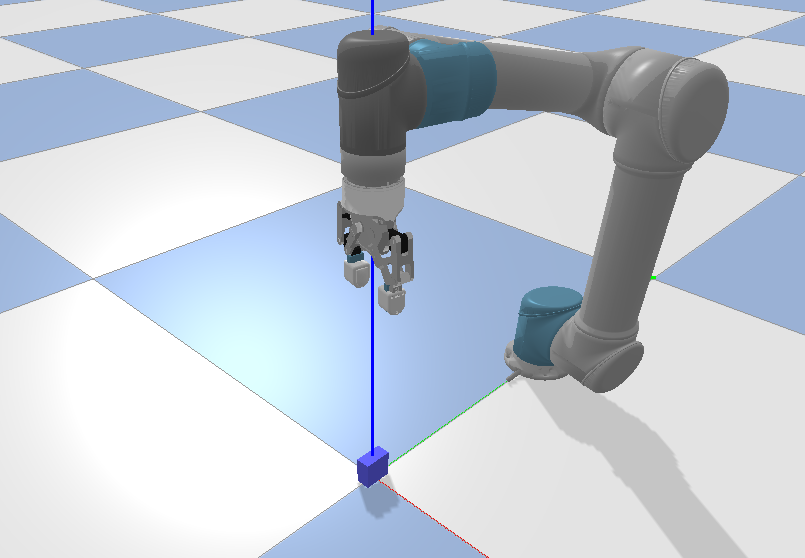
\includegraphics[width=7cm]{docs/Project Report/Media/4_1_2_init_config.png}\label{fig:4.1a}}}%
    \qquad
    \subfloat[\centering Move end effector to specific pose (with vertical padding)]{{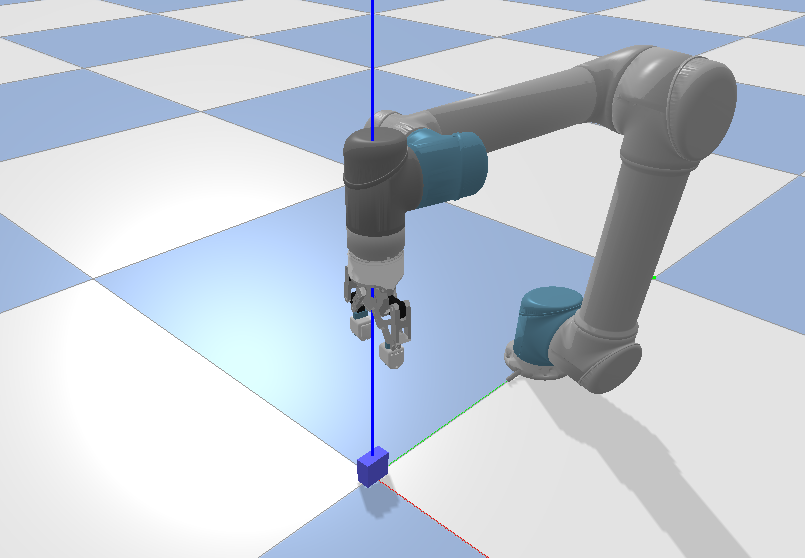
\includegraphics[width=7cm]{docs/Project Report/Media/4_1_2_ee_pose_with_pad.png}\label{fig:4.1b}}}%
    \qquad
    \subfloat[\centering Remove vertical padding and close gripper]{{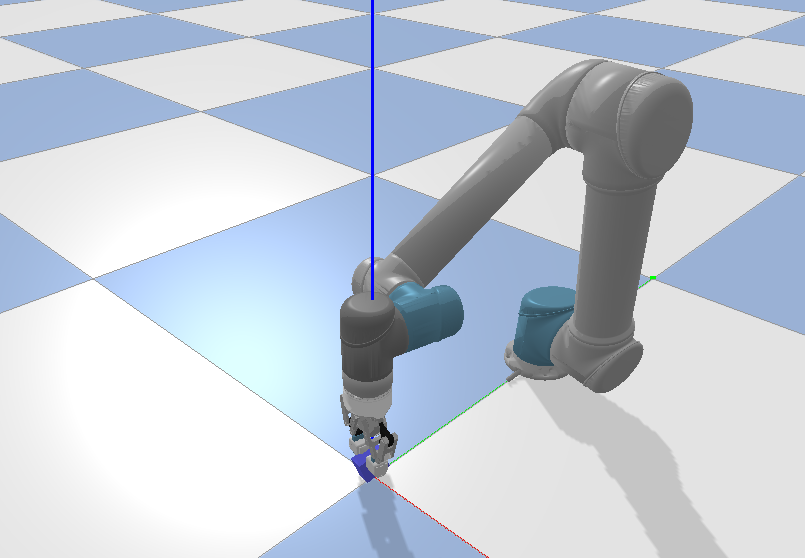
\includegraphics[width=7cm]{docs/Project Report/Media/4_1_2_ee_pose_no_pad.png}\label{fig:4.1c}}}%
    \qquad
    \subfloat[\centering Lift object]{{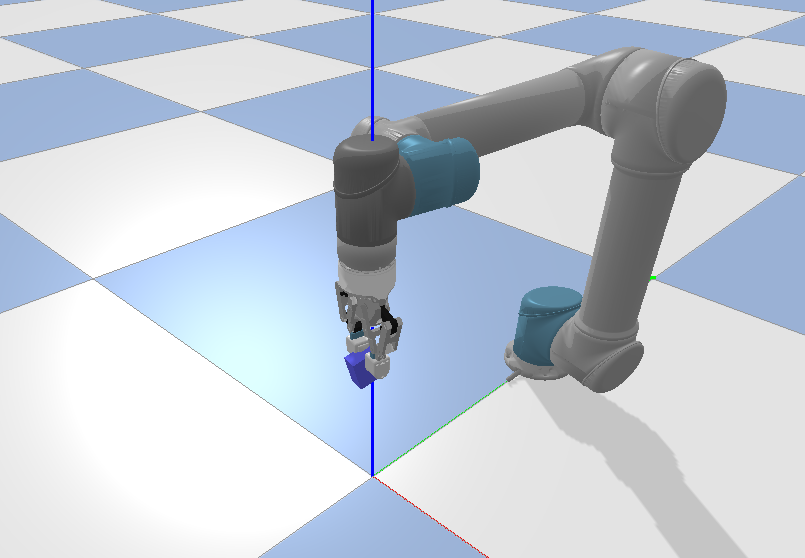
\includegraphics[width=7cm]{docs/Project Report/Media/4_1_2_pick_obj.png}\label{fig:4.1d}}}%
    \caption{Tactile and visual data collection procedure on a single generated hand pose}%
    \label{fig:4.1}%
\end{figure}

Before lifting the object, the robot measures the number of contact points between the two fingers and the object to ensure the grasp is stable. We define a grasp to be stable if there are a non-zero number of contact points, in which the robot records depth and color tactile information using the DIGIT \cite{Lambeta2020DIGIT} tactile sensors on each finger. The depth read We concatenate each pair of depth and color tactile readings into a $(160\times240)$ gray-scale image and a $(160\times240\times3)$ RGB image respectively.\\

After collecting the tactile readings, the robot performs a sanity check on the recorded depth tactile data. Since the color data is an RGB representation of the depth data, it does not require any additional checks. To facilitate the sanity check, we analyze whether the average pixel value exceeds a particular threshold. This process enables us to remove any erroneous signals (\ref{fig:4.2a}) and preserve the precise depth data (\ref{fig:4.2b}). By utilizing this method, we can enhance the quality of the data and ensure accurate lifting of the object.

\begin{figure}[H]%
    \centering
    \subfloat[\centering Invalid depth data]{{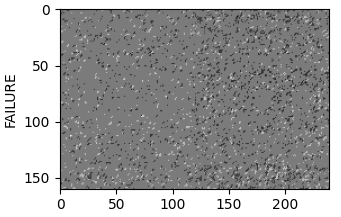
\includegraphics[width=7cm]{docs/Project Report/Media/4_1_2_failure_depth_data.png}\label{fig:4.2a}}}%
    \qquad
    \subfloat[\centering Valid depth data]{{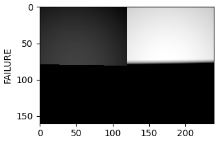
\includegraphics[width=7cm]{docs/Project Report/Media/4_1_2_valid_depth_data.png}\label{fig:4.2b}}}%
    \caption{Concatenated depth data for each finger}%
    \label{fig:4.2}%
\end{figure}

Once the robot verifies that the object is stably held (i.e. the tactile data is valid), it lifts the object vertically upwards by an offset of $p_z$ and holds the object for 750 steps (\ref{fig:4.1d}). Finally, the robot records a binary outcome of the grasp by determining if the change in the object's z-position $\Delta z$ is greater or equal to the vertical padding $p_z$:

\begin{equation}
    outcome=\begin{cases}1 & \Delta z\geq p_z \\ 0 & \Delta z<p_z\end{cases}
\end{equation}

After executing each random pose, we append the collected tactile data, end effector pose and grasp outcome to individual arrays. Once the required data for our $N$ random end effector poses has been collected, these arrays are saved to separate files which can be loaded for further analysis. Specifically, we create one .npy file each for the depth, color, grasp outcomes, and random pose data.


\newpage
\section{Visualising Hand Poses}
\label{sec:4.3}
Before we train our baseline model, we are interested if a clear decision boundary exists between successful and unsuccessful grasps. We create a visualisation of each hand pose $X_n$ in a 3-dimensional space, using its Cartesian coordinates and the "pitch-row-yaw" rotational matrix representation $R$ of its Euler angles ($\alpha,\beta,\gamma$) \cite{weisstein}:

\begin{equation}
    R=r_x\cdot(r_y\cdot r_z)
\end{equation}

\noindent where $r_x$, $r_y$ and $r_z$ are the rotational matrices about the $x$, $y$ and $z$-axis respectively:

\begin{figure}[H]
    \centering
    \begin{equation*}
        r_x = \begin{pmatrix}1&0&0 \\ 0&cos(\alpha)&sin(\alpha) \\ 0&-sin(\alpha)&cos(\alpha)\end{pmatrix}\;\;
        r_y = \begin{pmatrix}cos(\beta)&0&-sin(\beta) \\ 0&1&0 \\ sin(\beta)&0&cos(\beta)\end{pmatrix}\;\;
        r_z = \begin{pmatrix}cos(\gamma)&sin(\gamma)&0 \\ -sin(\gamma)&cos(\gamma)&0 \\ 0&0&1 \end{pmatrix}
    \end{equation*}
    \caption{Rotational matrices for each axis in the rotational matrix representation of Euler angles}
    \label{fig:4.3}
\end{figure}

\noindent Using this information, we annotate 20 random hand poses from our dataset in a 3-dimensional plot. Each 6D hand pose is represented using a skeleton 2-finger model, where green and red poses denote successful and unsuccessful grasps respectively:
\begin{figure}[H]%
    \centering
    \subfloat[\centering Orientation 1]{{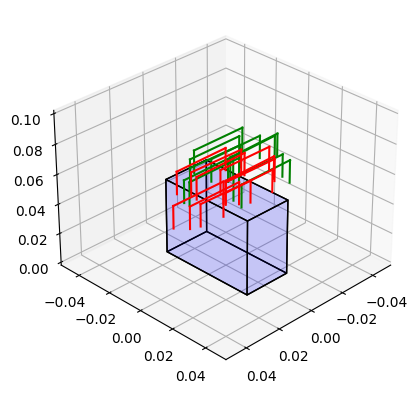
\includegraphics[width=6.5cm]{docs/Project Report/Media/hand_pose1.png} }}%
    \qquad
    \subfloat[\centering Orientation 2]{{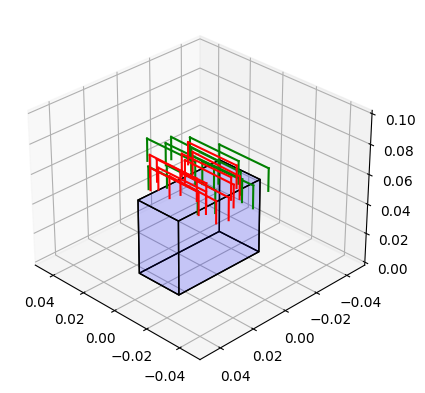
\includegraphics[width=6.5cm]{docs/Project Report/Media/hand_pose2.png} }}%
    \caption{Visualisation of 20 end effector poses}%
    \label{fig:4.4}%
\end{figure}
\noindent From the above figures, we are able to visually determine a rough decision boundary between successful (green) and unsuccessful (red) grasps. Therefore, we believe that it is feasible to fit this dataset using a simple binary classifier as our baseline approach.


\section{Feature Engineering \& Data Pre-processing}
\label{sec:4.4}
We aim to assess the efficacy of utilising our multi-modal dataset for our grasping task through experimenting with various combinations of the tactile and visual (random end effector poses) data.


\subsection{Multi-modal Data Combinations}
\label{sec:4.4.1}
In this project, we segregate our dataset into tactile-only, visual-only and concatenated tactile and visual datasets:
\begin{table}[H]
    \centering
    \begin{tabular}{|p{3cm}|p{4cm}|p{6cm}|}
        \hline
        Data Combination & Dimensions & Creation \\
        \hline
        Tactile only & $N\times160\times240\times4$ & Concatenating the depth ($N\times160\times240$) and color ($N\times160\times240\times3$) data \\
        \hline
        Visual only & $N\times6$ & Random 6D end effector poses \\
        \hline
        Tactile + Visual & $N\times(160\times240\times4+6)$ & Concatenating the flattened tactile-only and visual-only datasets \\
        \hline
    \end{tabular}
    \caption{Various segregated datasets}
    \label{tbl:4.1}
\end{table}


\subsection{Dimensionality Reduction}
\label{sec:4.4.2}
Due to the high dimensionality nature of our tactile and visual datasets, we experimented with two widely-used dimensionality reduction techniques, PCA and CNN feature extraction, to retain as much information as possible from the dataset.


\subsubsection{Principal Component Analysis (PCA)}
\label{sec:4.4.2.1}
For each image in the tactile and visual datasets, we select the top 2 eigenvectors that correspond to the largest eigenvalues as the principal components for the data.


\subsubsection{Convolution Neural Network (CNN) Feature Extraction}
\label{sec:4.4.2.2}
We create a 3-layer convolution neural network to extract the important features from our data combinations. Each convolution layer is interwined with a MaxPool2D layer with a $2\times2$ kernel. \hyperref[fig:4.5]{Fig 4.5} illustrates the architecture for the CNN we used:
\begin{figure}[H]
    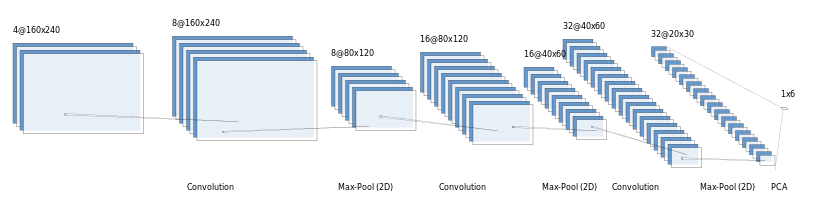
\includegraphics[scale=0.7]{docs/Project Report/Media/nn.png}
    \caption{Architecture for feature extraction CNN}
    \label{fig:4.5}
\end{figure}


\subsection{Data Pre-processing}
\label{sec:4.4.3}



\section{Baseline Model \& Training}
\label{sec:4.5}
Based on our findings (\hyperref[sec:4.3]{Section 4.3}), we propose a simple binary logistic regression (LR) classifier to predict the grasp outcome for a given random end effector pose. Ideally, this LR model is able to determine a decision boundary for segregating successful and unsuccessful grasp poses.\\

We train the classifier using the three discussed dataset combinations (\hyperref[sec:4.4.1]{Section 4.4.1}). Additionally, we apply a combination of dimensionality reduction techniques to these datasets discussed in (\hyperref[sec:4.4.2]{Section 4.4.2}), including ConvNet only and ConvNet with PCA (top $k=5$ principal components).


\subsection{Summary of training results}
\label{sec:4.5.1}
Table 4.2 shows the accuracy for each LR model trained based on the dataset type and preprocessing method
\begin{table}[H]
    \centering
    \small
    \begin{tabular}{lccccc}
        \toprule
        & \multicolumn{3}{c}{Dataset} & \multicolumn{2}{c}{Property of sample} \\
        \cmidrule{2-4}\cmidrule{5-6}
        Preprocessing & Visual only & Tactile only & Both & Shape & Dimensionality \\
        \midrule
        Raw & 51.25\% & 85.00\% & 85.00\% & 160x240x4 & 153600 \\
        CNN & -- & 83.75\% & 81.25\% & 64x10x15  & 9600 \\
        CNN + PCA ($k=5$) & -- & 78.75\% & 80.00\% & 5 & 5\\
        \bottomrule
    \end{tabular}
    \caption{Accuracy of LR model on dataset variations}
    \label{tbl:4.2}
\end{table}


\subsection{Balancing trade-off between accuracy and dimensionality}
\label{sec:4.5.2}
Based on the results presented in \hyperref[tbl:4.2]{Table 4.2}, we have determined that using both tactile and visual data together produces the highest accuracy for our LR models. While raw data performed better than other pre-processing techniques, we recognize that the dimensionality of the data must also be considered. Therefore, we have found that extracting features from our dataset using a ConvNet and selecting only the top $k=5$ components provides comparable accuracy with significantly lower dimensionality.


\section{Conclusion}
\label{sec:4.6}


\subsection{Feature Representation}
\label{sec:4.6.1}
Select the most promising representation and use it for actual generative model in Sec 4.


\subsection{Analysis of Results}
\label{sec:4.6.2}
Mention dimensionality constraints on computability costs!



%----------------------------------------------------------------------------------
% Section 5: Proposed Approach
%----------------------------------------------------------------------------------
\chapter{Multilayer Perceptron Artificial Neural Network for Grasp Stability Prediction}
\label{chap:5}

\section{Mutlilayer Perceptrons and Motivation}
\label{sec:5.1}
A multilayer perceptron (MLP) as a feedforward neural network consisting of a minimum of three fully-connected layers of perceptrons (neurons). Every MLP contains an input layer that receives input data, an output layer that produces a prediction based on patterns within the data, and at least one hidden layer that enable the MLP to learn complex representations of the data.\\

For robotic grasping on a specific object, there may exist certain grasp configurations that yield a high grasp stability and success rate. For instance, grasping an object around its center of gravity can minimise rotational forces on the object that could cause it to tilt, hence increasing the probability of a successful grasp. MLPs excel at learning non-linear relationships between input and output data. Therefore, intuitively, a MLP is a good candidate to learn such patterned configurations from the complex dataset and generalise them into a simple grasping strategy based on different object types.\\

To introduce robustness in robotic grasping for various object types, we trained our MLP model on three primitive object categories, namely rectangular boxes, cylinders, and bottle-shaped objects (which are more rigid than typical cylinders). Our intention is to explore the potential influence of an object's geometric characteristics, such as its width and height, on the model's accuracy.


\section{Dataset Collection and Representation}
\label{sec:5.2}


\subsection{Object Variations}
\label{sec:5.2.1}
To enhance the robustness of our model, we have trained it on three primitive object categories that collectively represent a sizable proportion of daily-life objects: rectangular boxes, cylinders and bottles. For each object category, we generate three instances with slightly different dimensions. The 3D meshes of these object variations and their dimensions are listed in \hyperref[tbl:5.1]{Table 5.1}.

\begin{table}[H]
    \centering
    \caption{3D meshes of all experimental object variations}
    \resizebox{\textwidth}{!}{%
        \begin{tabular}{lccccccccc}
            \toprule
            & 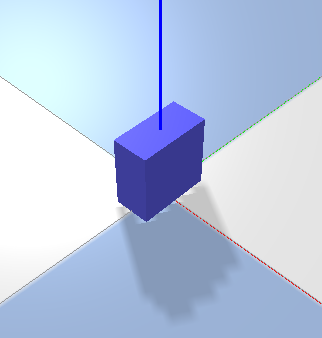
\includegraphics[width=0.1\textwidth]{docs/Project Report/Media/block1.png} & 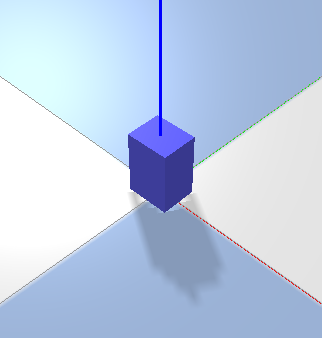
\includegraphics[width=0.1\textwidth]{docs/Project Report/Media/block2.png} & 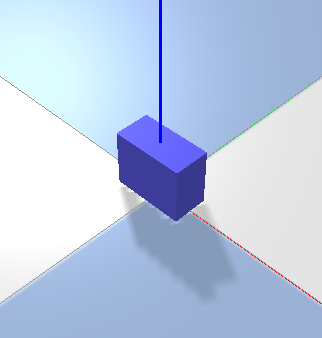
\includegraphics[width=0.1\textwidth]{docs/Project Report/Media/block3.png} &
            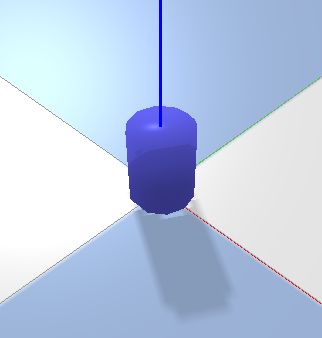
\includegraphics[width=0.1\textwidth]{docs/Project Report/Media/cylinder1.png} & 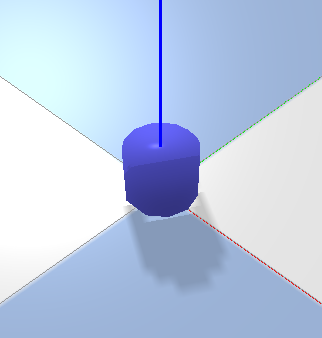
\includegraphics[width=0.1\textwidth]{docs/Project Report/Media/cylinder2.png} & 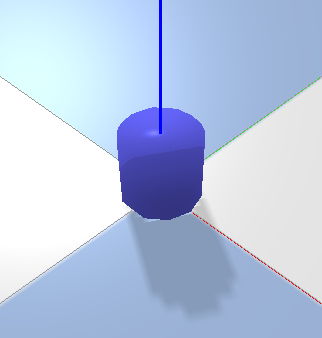
\includegraphics[width=0.1\textwidth]{docs/Project Report/Media/cylinder3.png} & 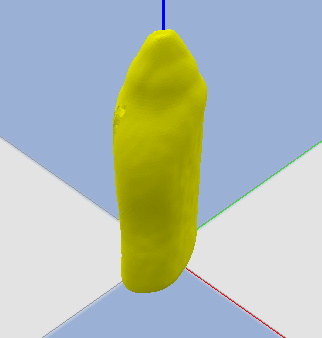
\includegraphics[width=0.1\textwidth]{docs/Project Report/Media/mustard_bottle1.png} & 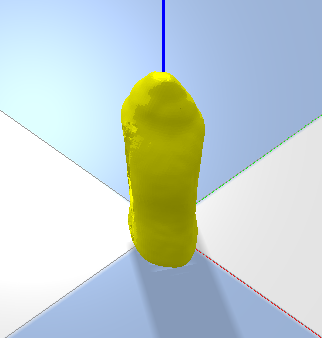
\includegraphics[width=0.1\textwidth]{docs/Project Report/Media/mustard_bottle2.png} &  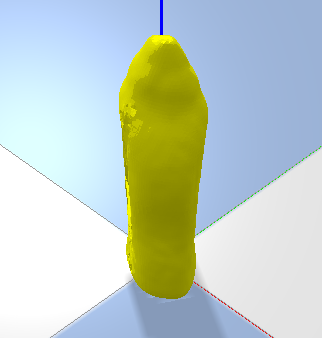
\includegraphics[width=0.1\textwidth]{docs/Project Report/Media/mustard_bottle3.png} \\
            & Block 1 & Block 2 & Block 3 & Cylinder 1 & Cylinder 2 & Cylinder 3 & Bottle 1 & Bottle 2 & Bottle 3 \\
            \midrule
            Depth  & 0.025 & 0.03  & 0.05  & 0.04 & 0.045  & 0.05  & 0.06 & 0.04 & 0.04 \\
            Width  & 0.05  & 0.025 & 0.025 & 0.04 & 0.045  & 0.05  & 0.04 & 0.06 & 0.06 \\
            Height & 0.05  & 0.045 & 0.04  & 0.05 & 0.035  & 0.045 & 0.04 & 0.06 & 0.04 \\
            Radius & --    & --    & --    & 0.02 & 0.0225 & 0.025 & --   & --   & --   \\
            \bottomrule
        \end{tabular}
    }
    \label{tbl:5.1}
\end{table}


\subsection{Data Collection}
\label{sec:5.2.2}
Utilising our Pybullet data collection pipeline from \hyperref[sec:4.2]{Section 4.2}, we collect multi-modal data for every object variation. Then, for each variation, we manually select $i=4$ seed poses and record the data of 20 successful and 20 unsuccessful grasps with Gaussian noise applied to the seed pose. This forms a dataset of 9x160=1440 grasps in total (720 stable and 720 unstable grasps) consisting tactile sensor readings and hand poses.


\subsection{Geometric Features of an Object}
\label{sec:5.2.3}
Each primitive object category in our dataset possesses unique characteristics. For instance, the curvature of an object's surface can differentiate cylinders and bottles from blocks with ease. As objects within a primitive class often share similar geometric features (such as the curvature of cylinders), our model could potentially generalize successful and unsuccessful grasp poses within each object category by establishing a connection between those poses and the object's properties.\\

To this end, we extracted and analysed several geometric features of the 9 object variations in order to determine which of them can effectively differentiate between the object categories.


\subsubsection{Principal Curvature}
\label{sec:5.2.3.1}
The principal curvatures of an object mesh is pair of maximum and minimum values of curvatures at each vertex of the mesh, expressed by the eigenvalues of the shape operator at that vertex \cite{enwiki:1141654906}. We investigate whether the top $k$ principal curvatures are able to categorize the object variations correctly.

\vspace*{-0.7cm}
\begin{figure}[H]%
    \centering
    \subfloat[\centering Top $k=2$ components; Variance captured: 91.43\%]{{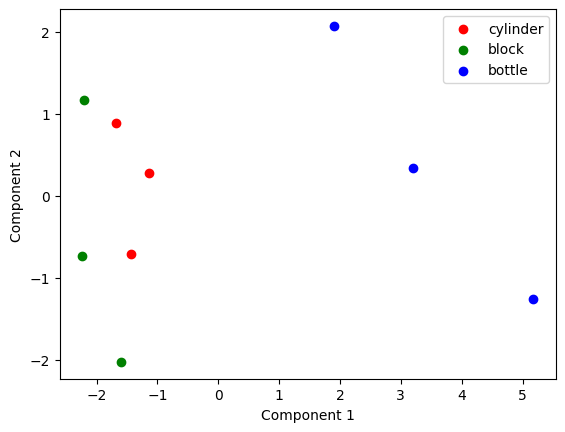
\includegraphics[width=0.4\textwidth]{docs/Project Report/Media/principal_curvature_2d.png} }}%
    \qquad
    \subfloat[\centering Top $k=3$ components; Variance captured: 97.34\%]{{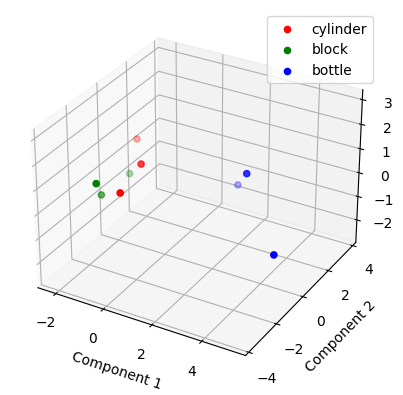
\includegraphics[width=0.4\textwidth]{docs/Project Report/Media/principal_curvature_3d.png} }}%
    \caption{Clustering using PCA-extracted components based on principal curvatures of objects}%
    \label{fig:5.1}%
\end{figure}

\hyperref[fig:5.1]{Figure 5.1} visualises the top $k=2$ and $k=3$ principal curvatures for all the object variations in our dataset. We found that the principal curvatures were able to:
\begin{enumerate}
    \item successfully cluster the object variations for each category
    \item capture a high amount of variance of the curvatures for all objects
\end{enumerate}
\noindent Thus, we conclude that principal curvatures is a valid representation of geometric features for our dataset of objects.


\section{Preprocessing}
\label{sec:5.3}
Based on our analysis results of our baseline approach in \hyperref[sec:4.7]{Section 4.7}, we concluded that under limited dimensionality circumstances, the Logistic Regression model fits the dataset with the highest accuracy using a convolutional neural network as a dimensionality reduction technique. Therefore, before training our MLP, we extract important features from our dataset using the same \hyperref[fig:4.5]{CNN} architecture. This results in a condensed dataset of shape $1200\times512$.\\

To improve the convergence speed and performance for training our MLP model, we normalise the tactile and visual datasets with zero mean and unit variance. This also prevents the initialisation of large weights during back-propagation.


\section{Training}
\label{sec:5.4}
We trained our MLP model on two versions of our dataset:
\begin{enumerate}
    \item tactile and visual data (end effector poses only)
    \item tactile and visual data (end effector poses and object geometric features)
\end{enumerate}


\subsection{Training details}
Split dataset into 80\% training and 20\% validation;


\subsection{Loss function}
simple binary cross-entropy with logits loss (sigmoid + bce loss in a single class)


\subsection{Optimizer}
Adam with lr=1e-3


\section{Validation}
\begin{figure}[H]%
    \centering
    \subfloat[\centering ]{{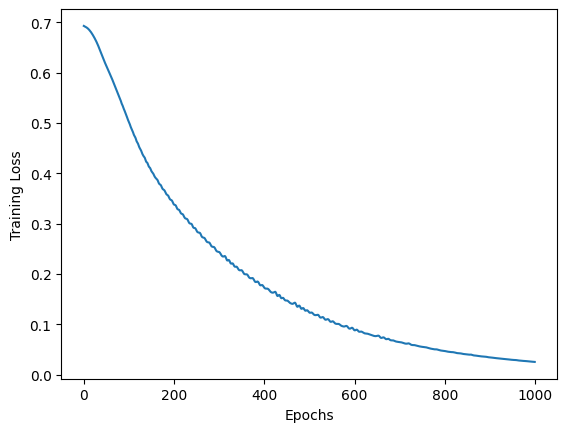
\includegraphics[width=7cm]{docs/Project Report/Media/mlp_no_geo_loss_curve.png}\label{fig:5.2a}}}%
    \qquad
    \subfloat[\centering ]{{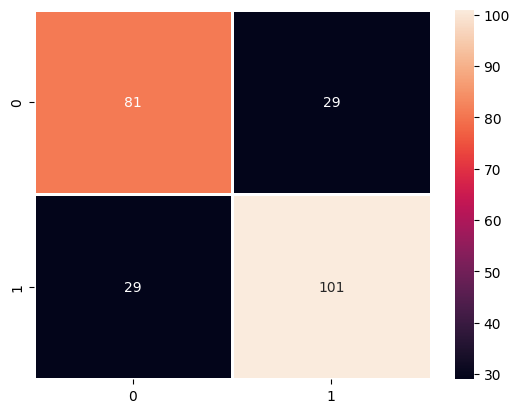
\includegraphics[width=7cm]{docs/Project Report/Media/mlp_no_geo_cm.png}\label{fig:5.2b}}}%
    \caption{Results for MLP without geometric features}%
    \label{fig:4.2}%
\end{figure}
Accuracy = 75.83\%

\begin{figure}[H]%
    \centering
    \subfloat[\centering ]{{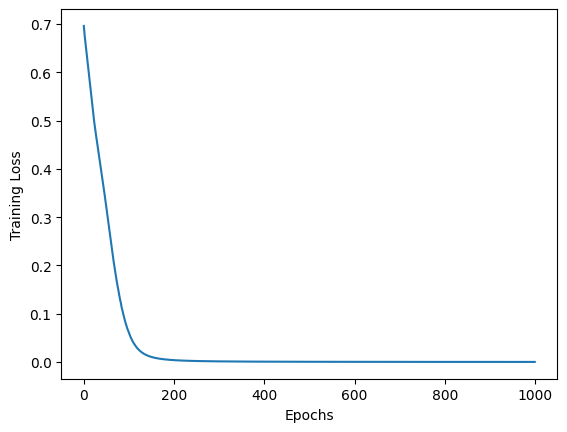
\includegraphics[width=7cm]{docs/Project Report/Media/mlp_geo_loss_curve.png}\label{fig:5.3a}}}%
    \qquad
    \subfloat[\centering ]{{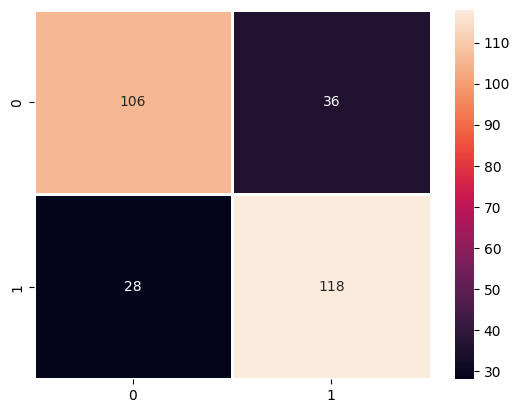
\includegraphics[width=7cm]{docs/Project Report/Media/mlp_geo_cm.png}\label{fig:5.3n}}}%
    \caption{Results for MLP with geometric features}%
    \label{fig:4.2}%
\end{figure}
Accuracy = 76.74\%


\section{Interesting experiments}
* in data collection, show grasp examples, good and bad grasps before and after lifting - after fingers are closed you completed the grasp - we want to show what is a good grasp, what a good grasp looks like, what a bad grasp looks like before we lift, then after we lift we want to show the reader what it means to be successful or fail.  
* visulize some examples tactile features from good and bad grasps 
* for PCA, choosing number of components, you plot the variance vs number of components, tactile feature selection? 


\begin{itemize}
\item train with data from 2 objects from each category. And test with data from remaining objects. 
 \begin{itemize}
\item randomly subsample the grasps, repeat the experiemtns 10 times.
\item repeat that for every object - (test objects:box1, cyl1, bot1, test2: box2, cyl2, bottle2 ...)
\item report using tactile only, vision only (hand poses + geometric features), all features

 \end{itemize}
    %\item Train with data of 2 blocks, test with data of 1 block
    \item Train with randomly chosen data from all types of objects (e.g. block + cylinder + bottles)

\begin{itemize}
\item randomly subsample the grasps across all objects, repeat the experiemtns 10 times.
\item report using tactile only, vision only (hand poses + geometric features), all features

\item plot the success rates versus data size - use all the features, all the objects, this is to show if the data size is good enough

\end{itemize}
    
\end{itemize}

Friday 14  - results complete (section 5.6), tables entered with the data that we have
Friday 21 - results complete with the new data, start writing the text, and adding plots, figures 
Friday 28 - write whole text for results section and method - Yasemin reads, gives feedback - Send Marc as well
Friday 5 - The rest of the report done - Yasemin reads, gives feedback
Friday 11 - Final touches



%----------------------------------------------------------------------------------
% Section 6: Future Work
%----------------------------------------------------------------------------------
\chapter{Future Work}
\label{chap:6}
Since Pybullet is no longer being maintained, consider to move to mujico



%----------------------------------------------------------------------------------
% Appendix section
%----------------------------------------------------------------------------------
\appendix
\printbibliography

\chapter{Other appendices, e.g., code listing}
Put your appendix sections here

\end{document}